\documentclass[11pt,a4paper]{article}
\usepackage[T1]{fontenc}
\usepackage{lmodern}
\usepackage[margin=1in]{geometry}
\usepackage{amsmath,amssymb,amsthm,mathtools}
\usepackage{booktabs,array,tabularx}
\usepackage{enumitem}
\usepackage{microtype}
\usepackage{xcolor}
\usepackage{tikz,pgfplots}
\pgfplotsset{compat=1.18}
\usepackage{hyperref}
\hypersetup{
  colorlinks=true,
  linkcolor=blue!45!black,
  citecolor=blue!45!black,
  urlcolor=blue!45!black,
  pdftitle={Four-Dimensional Stochastic PL Optimization: Stagewise Bounds and Limits of Recursive Constructions},
  pdfauthor={Colombo Team},
  pdfsubject={Finite-variance gradient oracles, discrete path complexity, and geometric obstructions}
}
\setlength{\parskip}{0.25em}
\setlength{\parindent}{1.2em}
\emergencystretch=1.5em
\setlist[enumerate]{leftmargin=*,itemsep=0.28em,topsep=0.35em}
\setlist[itemize]{leftmargin=*,itemsep=0.28em,topsep=0.35em}
\newcommand{\R}{\mathbb R}
\newcommand{\E}{\mathbb E}
\newcommand{\Prb}{\mathbb P}
\newcommand{\eps}{\varepsilon}
\newcommand{\one}{\mathbf 1}
\newcommand{\norm}[1]{\left\lVert #1\right\rVert}
\newcommand{\ip}[2]{\left\langle #1,#2\right\rangle}
\newcommand{\tO}{\widetilde O}
\newcommand{\tOmega}{\widetilde\Omega}
\newcommand{\tTheta}{\widetilde\Theta}
\newcommand{\profile}{\mathfrak C_4}
\DeclareMathOperator{\Crit}{Crit}
\DeclareMathOperator{\sgn}{sgn}
\newtheorem{theorem}{Theorem}[section]
\newtheorem{lemma}[theorem]{Lemma}
\newtheorem{proposition}[theorem]{Proposition}
\newtheorem{corollary}[theorem]{Corollary}
\theoremstyle{definition}
\newtheorem{definition}[theorem]{Definition}
\newtheorem{assumption}[theorem]{Assumption}
\theoremstyle{remark}
\newtheorem{remark}[theorem]{Remark}
\newcolumntype{Y}{>{\raggedright\arraybackslash}X}

\title{\bfseries Four-Dimensional Stochastic PL Optimization:\\[0.2em]
Stagewise Bounds and Limits of Recursive Constructions}
\author{Colombo Team\\[0.3em]
\small\href{mailto:colombo.2026@outlook.com}{\texttt{colombo.2026@outlook.com}}}
\date{November 23, 2026}

\begin{document}
\maketitle

\begin{abstract}
We study the oracle complexity of minimizing smooth
Polyak--\L{}ojasiewicz functions on $\R^4$ using conditionally unbiased
stochastic gradients with finite variance.  Combining robust gradient
descent with a known gradient-flow trapping routine yields the
accuracy-dependent upper profile
\[
 \profile(\eps)=\sum_{s=0}^{N-1}
 \min\!\left\{\kappa(1+q_s),\
               \kappa^{3/2}+\sqrt{\kappa}\,q_s\right\},
 \qquad
 q_s=\frac{\sigma^2}{\mu\,2^{-s}\Delta_0},
 \quad
 N=\left\lceil\log_2\frac{\Delta_0}{\eps}\right\rceil .
\]
We prove the stagewise composition, identify its exact switching
threshold, and quantify its advantage over using either routine at every
stage.  We also establish matching bounds, up to logarithms, for a
discrete path problem with nonuniform query costs and terminal subset
queries.  The passage from this discrete result to a matching
optimization lower bound requires additional geometric information.
We prove that an isolated degree-carrying port cannot be switched
between two states with nonvanishing gradients, and that a region
containing one nondegenerate minimum cannot replace a region without
critical points while preserving the boundary gradient.  A separate PL
argument shows that an ancestor-scale inactive value floor at an active
instance's minimizer forces gradient separation at the ancestor scale.
These obstructions invalidate the corresponding separated-interface
recursive construction.  The paper therefore establishes an upper
bound and a discrete complexity characterization, while leaving the
matching four-dimensional optimization lower bound open.
\end{abstract}

\noindent\textbf{Keywords.}
Polyak--\L{}ojasiewicz inequality; stochastic first-order optimization;
fixed-dimensional oracle complexity; relational adversary;
Brouwer degree.
\par
\begin{samepage}
\noindent\textbf{AI Usage.}
Nearly the entire research pipeline for this paper was carried out by
Colombo, powered by GPT-5.6 Sol.
\par
\end{samepage}

\section{Introduction}

The Polyak--\L{}ojasiewicz (PL) inequality relates the objective gap to
the norm of the gradient.  Together with smoothness, it guarantees
linear convergence of gradient descent even when the objective is
nonconvex \cite{karimi2016}.  This guarantee does not, however, settle
the information complexity of the problem in a prescribed dimension.
An algorithm in four dimensions can explore spatial structure that
a dimension-independent descent analysis does not use.  Conversely,
a lower bound based on an increasing number of hidden coordinates
does not automatically apply in $\R^4$.

The distinction becomes especially relevant with noisy gradients.
Write $\kappa=L/\mu$ for the condition number,
$N=\lceil\log_2(\Delta_0/\eps)\rceil$ for the number of accuracy stages,
and $Q=\sigma^2/(\mu\eps)$ for the final noise-to-gap ratio.
Two available strategies have different costs: robust descent scales
as $\tO(\kappa(N+Q))$, whereas four-dimensional gradient-flow trapping
scales as $\tO(\kappa^{3/2}N+\sqrt\kappa\,Q)$
\cite{ouwang2026}.  Their one-stage guarantees have the same input and
output requirements.  This permits a choice at each accuracy scale,
rather than a single choice before optimization begins.

Establishing a corresponding lower bound poses a different problem.
A discrete path can conceal the location of its terminal bin, and
nonuniform query costs can reproduce the two competing algebraic
terms.  To obtain a lower bound for optimization, one must realize
that path by one globally defined smooth PL function and simulate
every query to that function.  Local derivative estimates do not
alone establish this realization.  The boundary gradients must carry
consistent topological indices, and the proposed noise masking must
respect the actual gradient differences between all inputs.

\subsection{Contributions and scope}

Our first result is an explicit stagewise upper bound.  At gap scale
$\Delta$, the relevant noise level is $q=\sigma^2/(\mu\Delta)$, and the
algebraic cost is
\[
 \Phi_\kappa(q)
 =\min\{\kappa(1+q),\ \kappa^{3/2}+\sqrt\kappa\,q\}.
\]
The two terms agree exactly at $q=\sqrt\kappa$ when $\kappa>1$.
We prove the stagewise guarantee with a common logarithmic overhead,
give a closed formula for its sum, and show that the algebraic
advantage over a fixed choice of routine is at most
$\min\{N,(\sqrt\kappa+1)/2\}$.  The condition-number factor in this
comparison is asymptotically sharp.  This refines the explicit
accuracy dependence; it does not by itself establish a new minimax
lower bound.

Our second result concerns the discrete problem that motivates the
candidate lower profile.  For paths of length $K$, coarse terminal
bins of side $\sqrt K$, and scale-$s$ subset queries costing
$1+q/s^2$, we prove a randomized expected-cost lower bound
\[
 \Omega\!\left(
 \min\left\{K(1+q),\
 \frac{K^{3/2}+\sqrt K\,q}{1+\log^7(K+2)}\right\}\right).
\]
Path following and bin enumeration give the corresponding upper
bound without the logarithmic denominator.  The theorem includes
all bin-contained subsets allowed by the model, so a selector tree
cannot evade this discrete lower bound merely by exposing such
subsets.

Our third contribution identifies precise restrictions on a
continuous realization.  We give self-contained index arguments for
signed ports and child replacements, followed by a quantitative
obstruction linking inactive value floors to observable gradient
signals.  These restrictions show why the discrete theorem and an
abstract direct-sum argument do not certify the proposed recursive
PL family.  In particular, this paper does not claim
$T^*_{4,\delta}(\eps)=\tTheta(\profile(\eps))$.

\subsection{Related work and comparable bounds}

Yue, Fang, and Lin \cite{yue2023} prove a lower bound of
$\Omega(\kappa\log(\Delta_0/\eps))$ for deterministic first-order
algorithms in a dimension that may grow with the instance.
Their result distinguishes general PL optimization from strongly
convex optimization.  Its dimension and algorithm quantifiers
do not give a randomized lower bound in a prescribed dimension.

Ou and Wang \cite{ouwang2026} analyze conditional heavy-tailed
gradient noise.  We use the finite-variance specialization of their
fixed-dimensional results and, specifically, the gap-halving
contract in their trapping proof.  All theorem and equation
numbers refer to version~1.  Table~\ref{tab:comparison}
compares only results for the same four-dimensional model.

\begin{table}[tb]
\centering
\small
\renewcommand{\arraystretch}{1.22}
\begin{tabularx}{\linewidth}{@{}p{0.35\linewidth}p{0.12\linewidth}Y@{}}
\toprule
Result & Type & Bound in common notation\\
\midrule
Robust gradient descent
(\S\ref{sec:upper}; cf.\ \cite{ouwang2026})
& Upper & $\tO\bigl(\kappa N+\kappa Q\bigr)$\\
Gradient-flow trapping
\cite[Theorem 5.2(ii)]{ouwang2026}
& Upper & $\tO\bigl(\kappa^{3/2}N+\sqrt\kappa\,Q\bigr)$\\
Stagewise composition
(Theorem~\ref{thm:upper})
& Upper & $\tO\bigl(\sum_{s=0}^{N-1}\Phi_\kappa(q_s)\bigr)$\\
Fixed-dimensional lower bound
\cite[Theorem 5.1]{ouwang2026}
& Lower & $\Omega(N+Q)$\\
\bottomrule
\end{tabularx}
\caption{Comparable optimization bounds: $d=4$, global Euclidean PL,
$L$-Lipschitz gradients, conditional variance at most $\sigma^2$,
and success probability at least $3/4$.  The lower row assumes
$\kappa\ge6$ and $\eps\le c_0\Delta_0$; for bounded $Q$ its noise term
is absorbed by $N\ge1$.  Upper rows suppress logarithmic overhead.
The discrete path theorem is intentionally excluded: its query
model is different.}
\label{tab:comparison}
\end{table}

The geometric algorithmic background is the gradient-flow trapping
method of Bubeck and Mikulincer \cite{bubeck2020}.  Their problem is
approximate stationarity on a compact domain.  Their randomized
lower-bound analysis uses Aaronson's relational adversary
\cite{aaronson2006} and the low-predictability walks of
H\"aggstr\"om and Mossel \cite{haggstrom1998}.
We make the adaptations needed for nonuniform discrete query costs
explicit.  A reduction from those discrete ingredients to global PL
optimization remains a separate requirement.

\section{Model and notation}
\label{sec:model}

For $0<\mu\le L$ and $\Delta_0>0$, let
$\mathcal F_4(L,\mu,\Delta_0)$ consist of differentiable functions
$f:\R^4\to\R$ with $f^\star=\inf_x f(x)>-\infty$ such that
\begin{align}
 \norm{\nabla f(x)-\nabla f(y)}
 &\le L\norm{x-y}, \label{eq:smoothness}\\
 \norm{\nabla f(x)}^2
 &\ge2\mu\bigl(f(x)-f^\star\bigr) \label{eq:pl}
\end{align}
for every $x,y\in\R^4$.  A designated initial point $x_0$ satisfies
$f(x_0)-f^\star\le\Delta_0$.  The parameters $L,\mu,\Delta_0,\sigma$
are available to the algorithm; $f^\star$ is not.

Let $\mathcal F_{t-1}$ contain the algorithm's randomness and all
previous oracle replies.  At an $\mathcal F_{t-1}$-measurable query
$x_t$, an admissible oracle returns $G_t\in\R^4$ satisfying
\begin{equation}
 \E[G_t\mid\mathcal F_{t-1}]=\nabla f(x_t),
 \qquad
 \E[\norm{G_t-\nabla f(x_t)}^2\mid\mathcal F_{t-1}]
 \le\sigma^2.
 \label{eq:oracle}
\end{equation}
Fresh repeated calls at a fixed point may be taken conditionally
independent, as in the original model.  The elementary robust
estimator below also works under the displayed conditional moment
conditions alone.  The oracle supplies gradients only; it does not
supply exact function values.

For $0<\delta<1/2$, let $T^*_{4,\delta}(\eps)$ be the least
deterministic budget for which an adaptive randomized algorithm
returns $\widehat x$ with
\[
 \sup_{f\in\mathcal F_4(L,\mu,\Delta_0)}
 \sup_{\mathcal O\in\mathfrak O_\sigma(f)}
 \Prb\{f(\widehat x)-f^\star>\eps\}\le\delta .
\]
Expected-cost lower bounds will be stated explicitly when proved.
No restriction to iterates, linear spans, or a bounded query domain
is imposed.

Throughout the paper,
\begin{gather}
 \kappa=\frac L\mu,\qquad
 N=\left\lceil\log_2\frac{\Delta_0}{\eps}\right\rceil,\qquad
 \Delta_s=2^{-s}\Delta_0,\qquad
 q_s=\frac{\sigma^2}{\mu\Delta_s},\qquad
 Q=\frac{\sigma^2}{\mu\eps}, \label{eq:parameters}\\
 \Phi_\kappa(q)=
 \min\{\kappa(1+q),\ \kappa^{3/2}+\sqrt\kappa\,q\},
 \qquad
 \profile(\eps)=\sum_{s=0}^{N-1}\Phi_\kappa(q_s).
 \label{eq:profile}
\end{gather}
We assume $0<\eps<\Delta_0$, so $N\ge1$.  All unspecified constants
are numerical unless a dependence is stated.  The notation
$\tO,\tOmega,\tTheta$ suppresses polynomial factors in
$1+\log(2+\kappa)$, $1+\log(\Delta_0/\eps)$, and
$1+\log(1/\delta)$.  We retain $N$ explicitly whenever comparing
accuracy profiles.

\section{A stagewise upper bound}
\label{sec:upper}

We first establish the robust descent contract directly.  The second
contract is an imported algorithmic result, stated with its precise
source.  The composition then requires only a common gap invariant.

\subsection{Robust gradient estimates and descent}

\begin{lemma}[Finite-variance gradient estimation]
\label{lem:robust-mean}
At a fixed query point $x$, for every $\eta>0$ and
$0<\rho<1/2$, there is an estimator $\widehat g$ with
\[
 \Prb\{\norm{\widehat g-\nabla f(x)}>\eta
       \mid\text{history before estimation}\}\le\rho
\]
using at most
$C(1+\sigma^2/\eta^2)\log(4/\rho)$ oracle calls.
\end{lemma}

\begin{proof}
Use $k$ consecutive groups of
$b=\max\{1,\lceil32\sigma^2/\eta^2\rceil\}$ calls and take the
coordinatewise median of their means, with $k$ odd.
Conditional on the history before a group, its mean has each
coordinate's variance at most $\sigma^2/b$: cross terms vanish by
conditional unbiasedness.  Chebyshev's inequality gives probability
at most $1/8$ of a coordinate error larger than $\eta/2$.
This bound remains valid conditional on all preceding groups.
For any specified set of $j$ groups, the probability that all
$j$ are bad for that coordinate is therefore at most $8^{-j}$.
Consequently, the probability that at least half the groups are bad
is at most $2^k8^{-k/2}\le2^{-k/2}$.
Choose $k\ge2\log_2(4/\rho)$ and use a union bound over the four
coordinates.  Each median coordinate is then within $\eta/2$ of
the truth, so the Euclidean error is at most $\eta$.
The stated number of calls follows.
\end{proof}

\begin{proposition}[Robust descent contract]
\label{prop:descent-contract}
Suppose $f(x)-f^\star\le\Delta$.  There is a routine returning $x^+$
with gap at most $\Delta/2$, with conditional failure probability
at most $\rho$, using
\[
 C\kappa\left(1+\frac{\sigma^2}{\mu\Delta}\right)
 \log\frac{C(2+\kappa)}{\rho}
\]
calls.
\end{proposition}

\begin{proof}
Run $M=\lceil\kappa\log4\rceil$ updates
$x_{t+1}=x_t-\widehat g_t/L$.  At each update apply
Lemma~\ref{lem:robust-mean} with
$\eta^2=\mu\Delta/4$ and failure probability $\rho/M$.
On the event that all estimates are accurate, write
$e_t=\widehat g_t-\nabla f(x_t)$.  Smoothness gives the exact
inexact-gradient bound
\[
 f(x_{t+1})\le f(x_t)
       -\frac{\norm{\nabla f(x_t)}^2}{2L}
       +\frac{\norm{e_t}^2}{2L}.
\]
By PL, the gap after $M$ updates is at most
\[
 \left(1-\frac1\kappa\right)^M\Delta+
 \frac{\eta^2}{2\mu}
 \le\frac{\Delta}{4}+\frac{\Delta}{8}
 <\frac{\Delta}{2}.
\]
The conditional union bound gives failure probability at most
$\rho$.  Multiplying the estimator cost by $M$ proves the result.
\end{proof}

\subsection{The trapping contract}

\begin{lemma}[Four-dimensional trapping contract; imported]
\label{lem:trap-contract}
Under the same starting condition, a gradient-only routine returns
a point of gap at most $\Delta/2$ with conditional failure
probability at most $\rho$ using
\begin{equation}
 C H(\kappa,\rho)^4
 \left(\kappa^{3/2}
       +\sqrt\kappa\,\frac{\sigma^2}{\mu\Delta}\right),
 \qquad
 H(\kappa,\rho)=1+\log\frac{2+\kappa}{\rho},
 \label{eq:trap-contract}
\end{equation}
oracle calls.
\end{lemma}

\begin{proof}[Source and specialization]
This is the one-stage estimate in the proof of
\cite[Theorem 5.2(ii), equations (246)--(258)]{ouwang2026}.
Set $d=4$ and the moment exponent $\alpha=2$, so their
$k=d-1=3$ and $p_\alpha=2$.
With $J=C\lceil\log(2+\kappa)\rceil$, the two terms in their
equation (258) become
$(\kappa J)^{3/2}$ and $J^2(\kappa J)^{1/2}\sigma^2/(\mu\Delta)$.
Their confidence factor is logarithmic.  All these factors are
bounded by the common fourth power in \eqref{eq:trap-contract}.
Their stage begins with a gap bound $\Delta$ and halves it.
The geometric trapping proof is used here as an external result.
\end{proof}

\subsection{Composition with a common invariant}

\begin{theorem}[Stagewise upper bound]
\label{thm:upper}
For $0<\eps<\Delta_0$ and $0<\delta\le1/4$,
\begin{equation}
 T^*_{4,\delta}(\eps)
 \le C
 \left[1+\log\frac{(2+\kappa)(N+1)}{\delta}\right]^4
 \profile(\eps).
 \label{eq:main-upper}
\end{equation}
The routine uses robust descent at stages with
$q_s\le\sqrt\kappa$ and trapping at the remaining stages.
For $\kappa=1$, either branch can be used.
\end{theorem}

\begin{proof}
At stage $s$, maintain only the current point and the known bound
$f(x_s)-f^\star\le\Delta_s$.  Apply the indicated contract with
conditional failure probability $\delta/N$.
Both contracts have exactly this input invariant and return a
$\Delta_s/2=\Delta_{s+1}$ gap bound.  The choice depends only on
the known parameters.

For $\kappa>1$, direct subtraction gives
\begin{equation}
 \kappa(1+q)-\bigl(\kappa^{3/2}+\sqrt\kappa\,q\bigr)
 =\sqrt\kappa(\sqrt\kappa-1)(q-\sqrt\kappa).
 \label{eq:switching-threshold}
\end{equation}
Thus the selected algebraic cost is $\Phi_\kappa(q_s)$.
The common logarithmic factor in \eqref{eq:main-upper} dominates
the overhead of both contracts.  Summing the costs proves the
budget bound.  Conditional on every previous stage succeeding,
the next stage fails with probability at most $\delta/N$.
A union bound over the first failing stage therefore bounds the
total failure probability by $\delta$.
Finally $\Delta_N\le\eps$.
\end{proof}

The threshold in Theorem~\ref{thm:upper} compares the algebraic
profiles after a common overhead is factored out.  Different
implementation constants or logarithmic factors can change the
best practical switching point without changing the theorem.

\section{Interpreting and comparing the upper profile}
\label{sec:profile}

\subsection{The one-stage regimes}

Table~\ref{tab:stage-regimes} and Figure~\ref{fig:profile} describe
the \emph{upper-bound envelope}.  The regime dominated by
$\kappa^{3/2}$ between $q=\sqrt\kappa$ and $q=\kappa$ comes from the deterministic cost of
trapping; it is not an established minimax plateau.

\begin{table}[tb]
\centering
\small
\renewcommand{\arraystretch}{1.2}
\begin{tabularx}{\linewidth}{@{}p{0.25\linewidth}p{0.22\linewidth}Y@{}}
\toprule
Noise-to-gap ratio & $\Phi_\kappa(q)$ up to constants
& Selected mechanism\\
\midrule
$0\le q\le1$ & $\kappa$ & Descent; deterministic work dominates.\\
$1\le q\le\sqrt\kappa$ & $\kappa q$
& Descent; gradient estimation dominates.\\
$\sqrt\kappa\le q\le\kappa$ & $\kappa^{3/2}$
& Trapping; surface exploration dominates.\\
$q\ge\kappa$ & $\sqrt\kappa\,q$
& Trapping; stochastic surface estimation dominates.\\
\bottomrule
\end{tabularx}
\caption{Four regimes of the attainable one-stage profile for
$\kappa>1$.  Adjacent formulas agree up to constants at their
boundaries.  No optimization lower bound is asserted by this table.}
\label{tab:stage-regimes}
\end{table}

\begin{figure}[tb]
\centering
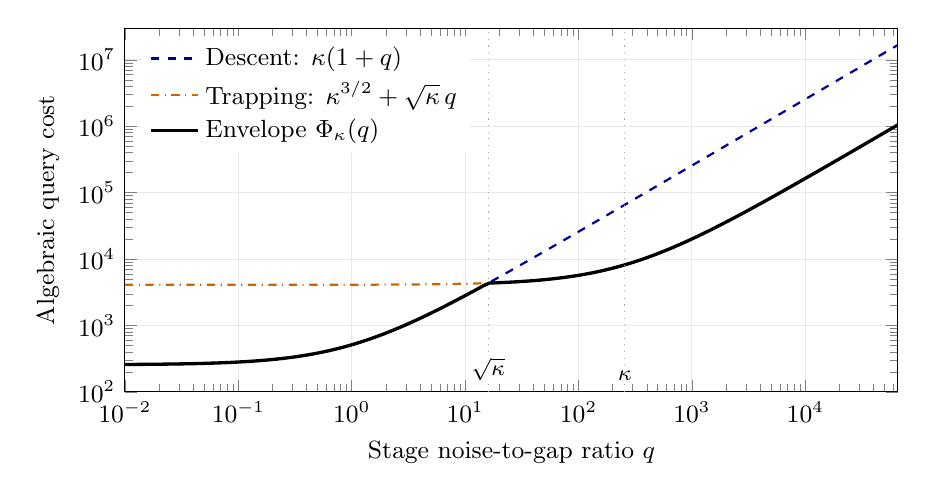
\begin{tikzpicture}
\begin{loglogaxis}[
 width=0.94\linewidth,height=6.2cm,
 xmin=0.01,xmax=65536,
 ymin=100,ymax=30000000,
 xlabel={Stage noise-to-gap ratio $q$},
 ylabel={Algebraic query cost},
 grid=major,
 major grid style={gray!18},
 tick label style={font=\small},
 label style={font=\small},
 legend style={font=\small,at={(0.02,0.98)},anchor=north west,
               draw=none,fill=white},
 legend cell align=left,
 samples=160,
 domain=0.01:65536,
 ]
 \addplot[blue!60!black,dashed,thick] {256*(1+x)};
 \addlegendentry{Descent: $\kappa(1+q)$}
 \addplot[orange!80!black,dashdotted,thick] {4096+16*x};
 \addlegendentry{Trapping: $\kappa^{3/2}+\sqrt\kappa\,q$}
 \addplot[black,very thick] {min(256*(1+x),4096+16*x)};
 \addlegendentry{Envelope $\Phi_\kappa(q)$}
 \draw[gray!70,dotted] (axis cs:16,100)--(axis cs:16,30000000);
 \draw[gray!70,dotted] (axis cs:256,100)--(axis cs:256,30000000);
 \node[anchor=south,font=\footnotesize,fill=white,inner sep=1pt]
 at (axis cs:16,130) {$\sqrt\kappa$};
 \node[anchor=south,font=\footnotesize,fill=white,inner sep=1pt]
 at (axis cs:256,130) {$\kappa$};
\end{loglogaxis}
\end{tikzpicture}
\caption{The exact upper envelope for the illustrative value
$\kappa=256$, with logarithmic overhead omitted.
The two routines cross at $q=16$.
The figure depicts attainable costs, not a proved minimax phase diagram.}
\label{fig:profile}
\end{figure}

\subsection{An exact formula for the stage sum}

Let $n$ be the number of stages with $q_s\le\sqrt\kappa$, and let
$\ell=N-n$.  If $\sigma=0$, set $n=N$.  If $\sigma>0$, then
\[
 n=\min\!\left\{N,\,
       \max\!\left\{0,\,
       1+\left\lfloor\log_2\frac{\sqrt\kappa}{q_0}\right\rfloor
       \right\}\right\}.
\]
Because $q_s=2^s q_0$, summing each affine branch gives the exact
identity
\begin{equation}
\begin{split}
 \profile(\eps)
 ={}&\kappa n+\kappa q_0(2^n-1)\\
    &+\kappa^{3/2}(N-n)
       +\sqrt\kappa\,q_0(2^N-2^n).
\end{split}
\label{eq:exact-stage-sum}
\end{equation}
An equality stage may be assigned to either branch.

For $\sigma>0$, the last stage satisfies
$Q/2\le q_{N-1}<Q$, and
$\sum_{s=0}^{N-1}q_s\asymp Q$.
If $\ell=0$, \eqref{eq:exact-stage-sum} therefore gives
$\profile(\eps)\asymp\kappa N+\kappa Q$.
If $\ell\ge1$, the descent-stage stochastic sum is
$O(\kappa^{3/2})$, which can be absorbed by the trapping-stage
deterministic term.  Hence
\begin{equation}
 \profile(\eps)\asymp
 \kappa(N-\ell)+\kappa^{3/2}\ell+\sqrt\kappa\,Q
 \qquad(\ell\ge1).
 \label{eq:stage-sum-asymptotic}
\end{equation}
For exact gradients, the identity is simply
$\profile(\eps)=\kappa N$.

\subsection{How much does switching improve the profile?}

Define the algebraic cost of a fixed choice of routine by
\begin{equation}
 \mathcal M
 =\min\!\left\{
       \sum_{s=0}^{N-1}\kappa(1+q_s),\
       \sum_{s=0}^{N-1}(\kappa^{3/2}+\sqrt\kappa\,q_s)
       \right\}.
 \label{eq:fixed-routine-profile}
\end{equation}

\begin{proposition}[Sharp comparison with a fixed routine]
\label{prop:sharp-switching}
For every dyadic stage sequence,
\begin{equation}
 1\le\frac{\mathcal M}{\profile(\eps)}
 \le\min\!\left\{N,\frac{\sqrt\kappa+1}{2}\right\}.
 \label{eq:switching-gain}
\end{equation}
For each fixed $\kappa>1$, there are dyadic sequences with
$N\to\infty$ for which the ratio converges to
$(\sqrt\kappa+1)/2$.
\end{proposition}

\begin{proof}
Put $r=\sqrt\kappa$, $A(q)=r^2(1+q)$, and
$B(q)=r^3+rq$.  For every $q\ge0$,
\[
 \max\{A(q),B(q)\}\le r\min\{A(q),B(q)\}.
\]
Thus
\[
 \profile(\eps)\le\mathcal M
 \le\frac12\sum_s(A(q_s)+B(q_s))
 \le\frac{r+1}{2}\profile(\eps).
\]
Monotonicity also gives
$\mathcal M\le N\min\{A(q_{N-1}),B(q_{N-1})\}
\le N\profile(\eps)$.

For sharpness, fix $r>1$ and take
$q_0=rN/(2^N-1)$.  Then $\sum_s q_s=rN$, so both totals in
\eqref{eq:fixed-routine-profile} equal $r^2(r+1)N$.
Only $O(\log N)$ stages have $q_s>r$, and the sum of the remaining
$q_s$ is $O(r)$.  Splitting at this threshold yields
\[
 \profile(\eps)=2r^2N+O(r^3\log N).
\]
The ratio tends to $(r+1)/2$.
\end{proof}

This comparison concerns the algebraic profiles before algorithmic
overhead is restored.  Moreover, the gain is at most
$N=\Theta(1+\log(\Delta_0/\eps))$.  Under the logarithmic convention
of this paper, stagewise switching refines the explicit profile
without changing the previously available upper-bound class.



\section{Matching bounds for the discrete path problem}
\label{sec:discrete}

This section concerns a finite query problem, independently of any smooth
optimization realization.  It identifies the cost of locating the terminal
bin of a path when queries may inspect either individual vertices or subsets
of a terminal bin.  The underlying unpredictable-path construction is due to
H\"aggstr\"om and Mossel~\cite{haggstrom1998}; the use of such paths with a
relational adversary follows Bubeck and Mikulincer~\cite[Appendix~B]{bubeck2020}.
Here the relation has quadratic prefix weights, and terminal queries have
scale-dependent costs.

\subsection{Paths, terminal bins, and query costs}

The low-predictability theorem supplies a nearest-neighbor process
$(S_t)_{t\ge0}$ on $\mathbb Z$, starting at zero, for which
\begin{equation}
 \sup_{v}\Prb\{S_{i+k}=v\mid S_0,\ldots,S_i\}
 \le C\frac{1+\log^2(k+1)}{k+1},\qquad k\ge1,
 \label{eq:one-dimensional-predictability}
\end{equation}
uniformly over every prefix of positive probability.  Apply
\cite[Theorem~1.4]{haggstrom1998} with the decreasing sequence
$h(k)=[1+\log^2(k+1)]^{-1}$, for which
$\sum_{k\ge1}h(k)/k<\infty$; see also
\cite[Theorem~18]{bubeck2020}.  Put $B_t=(S_t+t)/2$, so that
$B_t-B_{t-1}\in\{0,1\}$.  Take three independent copies and define
\[
 P_t=(t,B_t^{(1)},B_t^{(2)},B_t^{(3)}),\qquad 0\le t\le m.
\]
Thus each increment belongs to the fixed alphabet
$\{1\}\times\{0,1\}^3$.  In particular, the first coordinate identifies the
time level.  A prefix of $P$ reveals exactly the corresponding prefixes of
the three copies, so independence and
\eqref{eq:one-dimensional-predictability} give
\begin{equation}
 \Prb\{P_{i+k}=v\mid P_0,\ldots,P_i\}
 \le C\frac{\log^6(k+2)}{(k+1)^3}.
 \label{eq:cubic-predictability}
\end{equation}
Write $\nu$ for the resulting distribution on its finite support
$\mathcal P_m$.

Partition the terminal lattice $\{m\}\times\{0,\ldots,m\}^3$ into bins of
side length $b$ in the last three coordinates.  Every bin contains at most
$b^3$ vertices, including bins truncated at the boundary.  The required
output is the bin $Y(P)$ containing $P_m$.
For a parameter $q\ge0$, the oracle accepts the following queries:
\begin{enumerate}
 \item A vertex query $(\ell,v)$, $0\le\ell<m$, returns
 $\one\{P_\ell=v\}$ and costs $1+q$.
 \item A terminal query $(A,s)$ returns $\one\{P_m\in A\}$, where $A$ is
 contained in one bin, $|A|\le C_A s^3$, and
 $s\in\{1,2,4,\ldots,b\}$.  Its cost is $1+q/s^2$.
\end{enumerate}
Here $C_A\ge1$ is a fixed constant and $b$ is a power of two.  The scale
$s$ is part of the query label.  This permissive model allows all subsets
meeting the displayed cardinality bound, not just geometric subcubes.
In particular, full-bin queries are permitted at scale $s=b$.

Set $\Lambda_m=1+\log^7(m+2)$.  The following elementary consequence of
\eqref{eq:cubic-predictability} will control all terminal queries at once.

\begin{lemma}[Terminal subset mass]
\label{lem:subset-mass}
For every allowed $(A,s)$ and every realized prefix ending at time $m-k$,
\[
 \Prb\{P_m\in A\mid P_0,\ldots,P_{m-k}\}
 \le \min\left\{1,
 C s^3\frac{\log^6(k+2)}{(k+1)^3}\right\}.
\]
For any fixed path $P\in\mathcal P_m$, the conditional probabilities along
its successive prefixes consequently satisfy
\[
 \sum_{k=1}^m k^2
 \Prb\{X_m\in A\mid X_{0:m-k}=P_{0:m-k}\}
 \le C s^3\Lambda_m,\qquad X\sim\nu.
\]
\end{lemma}

\begin{proof}
Sum \eqref{eq:cubic-predictability} over $A$.  For the second claim use
$k^2/(k+1)^3\le1/(k+1)$ and
$\sum_{k=1}^m\log^6(k+2)/(k+1)\le C\Lambda_m$.
\end{proof}

\subsection{A distributional adversary with variable query costs}

We state the adversary in a distributional form because that form also
supports independent composition.  The input set below is finite; algorithms
may be randomized and may have an unbounded stopping time of finite expected
cost.

\begin{lemma}[Costed relational adversary]
\label{lem:costed-adversary}
Let $w(x,y)$ be a nonnegative symmetric relation supported on input pairs
with different required outputs.  Define
\[
 T(x)=\sum_y w(x,y),\qquad
 T(x,a)=\sum_{y:A_y(a)\ne A_x(a)}w(x,y),
 \qquad W=\frac12\sum_xT(x)>0.
\]
Give input $x$ probability $\pi(x)=T(x)/(2W)$.  Queries have positive costs
$c(a)$.  Put
\[
 M=\inf_{\substack{w(x,y)>0\\A_x(a)\ne A_y(a)}}
 c(a)\max\left\{\frac{T(x)}{T(x,a)},
                 \frac{T(y)}{T(y,a)}\right\}.
\]
If an algorithm has average error at most $\eta<1/2$ under $\pi$, then
\begin{equation}
 \E_{\pi}[\operatorname{cost}]
 \ge \frac{1-2\eta}{2}\,M.
 \label{eq:robust-adversary}
\end{equation}
The expectation includes the algorithm's randomness.  The same statement
holds when the algorithm receives additional randomness independent of its
input.
\end{lemma}

\begin{proof}
First fix the internal random seed.  At a decision-tree node let $S$ be the
inputs reaching that node and let $a$ be its query.  A related pair in $S$
is separated there if its two answers differ.  Orient each such pair toward
an endpoint $z$ with
$T(z,a)/T(z)\le c(a)/M$, which exists by the definition of $M$.
The total weight of pairs oriented toward $z$ is at most $T(z,a)$.
Consequently the relation weight first separated at this node is at most
\[
 \frac{c(a)}{M}\sum_{z\in S}T(z).
\]
Summing over nodes bounds the total separated weight by
$(2W/M)\E_\pi[\operatorname{cost}]$.

At any leaf, two unseparated related inputs have different required outputs,
so at least one is misclassified.  The surviving relation weight is therefore
at most $\sum_{x\text{ misclassified}}T(x)$.  After averaging over the seed,
this is at most $2W\eta$.  Thus the expected separated weight is at least
$(1-2\eta)W$, proving \eqref{eq:robust-adversary}.  Nonnegative summation
justifies the same argument for finite expected cost.  Independent auxiliary
randomness can be included in the seed.
\end{proof}

This is a costed version of the relational method of
Aaronson~\cite{aaronson2006}; the explicit row distribution and error constant
make the required robustness transparent.

\subsection{The weighted path relation}

For $P,R\in\mathcal P_m$ with $Y(P)\ne Y(R)$, define
\begin{equation}
 w(P,R)=\nu(P)\sum_{i=0}^{m-1}(m-i)^2
 \Prb\{X=R\mid X_{0:i}=P_{0:i}\},\qquad X\sim\nu,
 \label{eq:path-relation}
\end{equation}
and set $w(P,R)=0$ otherwise.  For each common prefix, the corresponding
summand equals $(m-i)^2\nu(P)\nu(R)/\nu(P_{0:i})$; it vanishes when the
prefixes differ.  Hence $w$ is symmetric.

\begin{lemma}[Row mass and query disagreement]
\label{lem:relation-estimates}
There are universal constants $c_1,c_2,C>0$ such that, if
$b^3\Lambda_m\le c_1m^3$, then
\[
 T(P)\ge c_2\nu(P)m^3\qquad(P\in\mathcal P_m).
\]
If a vertex query $(\ell,v)$ is missed by $P$, and $r=m-\ell$, then
\[
 T(P,(\ell,v))\le C\nu(P)(r^2+\Lambda_m).
\]
If a terminal query $(A,s)$ is missed by $P$, then
\[
 T(P,(A,s))\le C\nu(P)s^3\Lambda_m.
\]
\end{lemma}

\begin{proof}
Before deleting same-bin pairs, the row mass is
$\nu(P)\sum_{k=1}^m k^2\ge\nu(P)m^3/3$.
Lemma~\ref{lem:subset-mass}, applied to the bin of $P_m$, bounds the deleted
mass by $C\nu(P)b^3\Lambda_m$.  Choosing $c_1$ sufficiently small proves
the first claim.

For a missed vertex at level $\ell$, only prefixes ending before $\ell$
can contribute.  With $k=\ell-i$ and $r=m-\ell$,
\begin{align*}
 T(P,(\ell,v))
 &\le C\nu(P)\sum_{k=1}^{\ell}
        (r+k)^2\frac{\log^6(k+2)}{(k+1)^3}\\
 &\le C\nu(P)\left[
 r^2\sum_{k=1}^{\infty}\frac{\log^6(k+2)}{(k+1)^3}
 +\sum_{k=1}^m\frac{\log^6(k+2)}{k+1}\right].
\end{align*}
The infinite series is finite, and the second sum is $O(\Lambda_m)$.
The terminal estimate follows directly from Lemma~\ref{lem:subset-mass}.
\end{proof}

\begin{theorem}[Discrete one-stage lower bound]
\label{thm:one-stage-discrete}
Let $K=4^p$, $m=K$, and $b=\sqrt K$.  For all sufficiently large $K$ there
is an input distribution $\pi_K$, independent of $q$, such that every
algorithm with average error at most $\eta<1/2$ in identifying $Y(P)$ has
expected query cost at least
\begin{equation}
 c(1-2\eta)
 \min\left\{K(1+q),
       \frac{K^{3/2}+\sqrt K\,q}{\Lambda_K}\right\}.
 \label{eq:discrete-stage-bound}
\end{equation}
In particular, the same lower bound holds for worst-case error at most
$\eta$ and worst-case expected cost.
\end{theorem}

\begin{proof}
Use the row distribution of \eqref{eq:path-relation}.
The row-mass condition holds for large $K$ because
$b^3\Lambda_K/K^3=\Lambda_K/K^{3/2}\to0$.
For any separated pair, at least one path misses the query.  For a vertex
query, Lemma~\ref{lem:relation-estimates} gives the adversary ratio
\[
 \frac{T(P)}{T(P,a)}\ge
 \frac{cm^3}{r^2+\Lambda_m}\ge cm.
\]
The last inequality uses $r\le m$ and
$\Lambda_m\le m^2$ for all sufficiently large $m$.
Multiplying by the query cost gives $cm(1+q)$.
For a terminal query of scale $s$, the costed ratio is at least
\[
 \frac{cm^3}{\Lambda_m}
 \left(s^{-3}+q s^{-5}\right).
\]
This expression decreases with $s$, so its minimum over the allowed scale
labels is attained at $s=b$.  Substituting $m=K$ and $b=\sqrt K$, and using
Lemma~\ref{lem:costed-adversary}, proves \eqref{eq:discrete-stage-bound}.
\end{proof}

The last monotonicity statement concerns the lower-bound expression.
It does not assert that a full-bin answer simulates all smaller subset
answers.  What the theorem establishes is that allowing every bin-contained
subset query at the specified cost does not invalidate
\eqref{eq:discrete-stage-bound}.  Turning this discrete result into an
optimization lower bound would require a separate, valid realization and
oracle simulation.

\begin{proposition}[Matching elementary upper bounds]
\label{prop:discrete-upper}
In the same discrete model, a deterministic algorithm identifies the
terminal bin with cost at most
\[
 C\min\{K(1+q),K^{3/2}+\sqrt K\,q\}.
\]
Consequently its randomized minimax expected cost at any fixed error
$\eta<1/2$ is determined up to the factor $\Lambda_K$.
\end{proposition}

\begin{proof}
Knowing $P_t$, test the at most eight possible successors to determine
$P_{t+1}$.  Use vertex queries before the terminal layer and singleton
terminal queries at scale one in the last layer.  This costs at most
$8K(1+q)$ and recovers the entire path.
Alternatively, query every terminal bin at scale $b=\sqrt K$ until finding
the bin containing the endpoint.  There are at most
$\lceil(K+1)/b\rceil^3\le C K^{3/2}$ bins, and each query costs $1+q/K$.
Choose the cheaper procedure.
\end{proof}

Let $R_{\rm path}(K,q)$ denote the smallest worst-case expected cost among
randomized algorithms whose error is at most $1/3$ on every path input.
Combining the last two results gives the precise discrete comparison
\begin{equation}
 \frac{c}{\Lambda_K}\Phi_K(q)
 \le R_{\rm path}(K,q)\le C\Phi_K(q),\qquad
 \Phi_K(q)=\min\{K(1+q),K^{3/2}+\sqrt K\,q\}.
 \label{eq:discrete-matching}
\end{equation}


\section{Topological obstructions to local assembly}
\label{sec:topological-obstructions}

The discrete path problem does not by itself supply a smooth objective.
A continuous realization must also transport the index of its eventual
minimum through every interface.  We record two obstructions to a proposed
realization: a degree-carrying port cannot be switched independently inside
a region with nonvanishing gradient, and a child containing one minimum
cannot replace a child with no critical point while preserving the entire
boundary gradient.  These statements concern particular assembly rules.
They do not rule out a selector whose interior changes jointly with its
ports, or determine whether the candidate complexity profile is attainable.

\subsection{Boundary index and a specified signed port}

Let $D\subset\mathbb R^4$ be a bounded smooth domain, oriented by the
ambient orientation, and let $f$ be smooth on a neighborhood of
$\overline D$.  Assume that $\nabla f$ does not vanish on $\partial D$.
Write
\[
 \mathcal I_D(f)
 :=\deg\left(\frac{\nabla f}{\|\nabla f\|}:
                   \partial D\longrightarrow S^3\right),
\]
where $\partial D$ has the outward boundary orientation.  If the boundary
has several components, the displayed degree is the sum of their degrees.
Equivalently, this is the Brouwer degree
$\deg(\nabla f,D,0)$.  The two consequences used below are
\begin{align}
 \nabla f\ne0\text{ on }\overline D
       &\quad\Longrightarrow\quad \mathcal I_D(f)=0,
       \label{eq:zero-free-index}\\
 \mathcal I_D(f)
       &=\sum_{x\in D:\,\nabla f(x)=0}
                      \operatorname{sgn}\det\nabla^2 f(x)
       \label{eq:critical-point-index}
\end{align}
when the critical points in the second line are nondegenerate.  In
particular, a unique nondegenerate minimum has index $+1$.

For completeness, these identities follow by deleting small disjoint
balls about the zeros of $\nabla f$.  The normalized gradient extends over
the remaining domain, so its degree on the outer boundary equals the sum
of its degrees on the small spheres.  With no zeros the sum is empty.
Near a nondegenerate zero, the gradient is homotopic on a sufficiently
small sphere to its invertible linearization $\nabla^2 f(x)$; the degree
of that linear map is the sign of its determinant.

The center of a port does not determine its relative degree.  A sign
specified only near the center leaves open how the field returns to a
common boundary field near the rim.  We therefore fix that return
explicitly.

\begin{definition}[A common-rim signed port]
\label{def:common-rim-port}
Consider a flat boundary patch with orthonormal coordinates $(s,y)$,
where $y\in B^3(0,1)$, $D$ lies on the side $s<0$, and increasing $s$
points out of $D$.  Choose the tangential coordinates so that the frame
$(s,y_1,y_2,y_3)$ preserves the ambient orientation.  Fix a smooth radial
cutoff $\chi$ satisfying
\[
 0\le\chi\le1,\qquad
 \chi(y)=1\quad(\|y\|\le1/3),\qquad
 \chi(y)=0\quad(\|y\|\ge2/3).
\]
For $\tau\in[-1,1]$, define the local potential
\begin{equation}
 J_\tau(s,y)
   =c+s\bigl[1-\chi(y)+\tau\chi(y)\bigr]
                 +\tfrac12\|y\|^2.
 \label{eq:completed-signed-germ}
\end{equation}
The negative and positive port states are $J_{-1}$ and $J_{+1}$.
They have respective germs $c-s+\|y\|^2/2$ and
$c+s+\|y\|^2/2$ near the port center, and they agree to all orders in a
collar of its rim.  A standard port replacement means this specified
replacement, up to orientation-preserving rigid changes of coordinates and
positive spatial and value rescalings.
\end{definition}

At $s=0$, the associated boundary vectors are
\begin{equation}
 v_\tau(y)=\nabla J_\tau(0,y)
       =\bigl(1-\chi(y)+\tau\chi(y),\ y\bigr).
 \label{eq:port-boundary-homotopy}
\end{equation}
Both endpoint fields are nonvanishing.  The endpoint potentials also have
nonvanishing gradients on a sufficiently thin port collar: their
longitudinal derivatives are $\pm1$ in the inner core, and on the cutoff
annulus their transverse derivatives are uniformly close to $y$ when
the collar is thin enough.  Thus the definition uses legitimate local
gradient fields.  It does not presuppose an extension over the rest of
$D$.

\begin{proposition}[Index change of one signed port]
\label{prop:signed-port-index}
Let $f_-$ and $f_+$ have nonvanishing gradients on $\partial D$.
Suppose their boundary gradients agree off one flat port and equal
$v_{-1}$ and $v_{+1}$, respectively, on that port, with the common-rim
convention of Definition~\ref{def:common-rim-port}.  Then
\begin{equation}
 \mathcal I_D(f_+)-\mathcal I_D(f_-)=1.
 \label{eq:single-port-index-change}
\end{equation}
Consequently, $N$ disjoint replacements with this orientation change the
index by $N$.  Reversing a replacement changes its contribution to $-1$.
\end{proposition}

\begin{proof}
Use \eqref{eq:port-boundary-homotopy} on the port and the unchanged
boundary gradient elsewhere to define a vector field
$H$ on $[-1,1]\times\partial D$.  The construction is smooth across the
rim because $\chi$ vanishes there.  Its only zero is
$(\tau,y)=(0,0)$: a zero requires $y=0$, where the first coordinate is
$\tau$.  In the oriented local coordinates $(\tau,y)$, its derivative
at that zero is the $4\times4$ identity matrix.

Remove a small four-dimensional ball about this zero.  On the remaining
product manifold $H/\|H\|$ maps continuously to $S^3$.  The degree on
its boundary is zero.  Its top and bottom faces contribute
$\mathcal I_D(f_+)$ and $-\mathcal I_D(f_-)$, while the newly created
inner sphere contributes $-1$, because the zero has positive local
degree.  Hence
$\mathcal I_D(f_+)-\mathcal I_D(f_-)-1=0$.
For several disjoint ports, perform the replacements one at a time and
sum the index changes.
\end{proof}

The explicit rim convention matters.  If only the two central germs are
specified, additional changes on the surrounding annulus can alter the
relative degree.  In that case one cannot infer an index change from the
central signs alone.  A construction that uses signed ports to count or
transport minima must specify which relative boundary class each port
represents.

\subsection{A single switch cannot be isolated}

\begin{corollary}[No independent zero-free sign switch]
\label{cor:no-isolated-switch}
There do not exist two smooth functions on the same ported domain that
both have nonvanishing gradients on its closure, agree in boundary
gradient except at one port, and differ at that port by a standard signed
replacement.
\end{corollary}

\begin{proof}
Both functions would have boundary index zero by
\eqref{eq:zero-free-index}, whereas
Proposition~\ref{prop:signed-port-index} makes their indices differ by
one.
\end{proof}

For example, consider two states of a cylindrical adapter with a common
output germ and common lateral jets.  If its input changes from negative
to positive in the common-rim sense, the two adapter states cannot both
be free of critical points.  The conclusion applies irrespective of the
adapter's scale or the values of its smoothness bounds.  A transverse
perturbation may keep the gradient nonzero in the central part of the
adapter, but that calculation alone does not establish that the
perturbation can return to the same lateral field without a zero or an
additional boundary change.

This distinction also applies to a selector with several input ports
and one output port.  In a valid routing state, the changes at a selected
input and at the output may have opposite relative indices, so their
total boundary-index change is zero.  Such cancellation is compatible
with a zero-free selector.  It does not justify implementing each change
in a separate zero-free adapter.

\begin{proposition}[Necessary coupling of port changes]
\label{prop:coupled-port-changes}
Suppose two zero-free selector states differ by one degree-carrying
input replacement and one degree-carrying output replacement of opposite
sign.  Their changes cannot be confined to two disjoint adapter domains
such that, on the boundary of either adapter, the fields agree except at
its designated external port.
\end{proposition}

\begin{proof}
Restrict the two functions to either adapter domain.  Their gradients
remain nonvanishing, and their boundary fields differ by exactly one
standard replacement.  This contradicts
Corollary~\ref{cor:no-isolated-switch}.
\end{proof}

Thus a selector based on signed-port transport needs a construction in
which the state changes are coupled through the interior or through
additional changing interfaces.  The proposition does not exclude such
a construction.  In particular, a constant-branch cell may depend on all
of its constantly many input bits; the dependence itself is compatible
with a local discrete-query model.  What remains necessary is an actual
scalar potential with the claimed boundary jets, gradient guard, and
query locality.  Finiteness of the state set supplies uniform constants
only after the required functions have been constructed.

\subsection{A common-boundary child cannot acquire one minimum}

The second obstruction does not depend on a choice of port model.
It follows directly from equality of the complete boundary gradients.

\begin{theorem}[Obstruction to an active/inactive child replacement]
\label{thm:common-boundary-child-obstruction}
Let $A$ and $I$ be smooth functions on a neighborhood of the closure of
the same bounded smooth domain $D$.  The following properties cannot
hold simultaneously:
\begin{enumerate}
\item $\nabla A=\nabla I\ne0$ on $\partial D$;
\item $A$ has exactly one critical point in $D$, and it is a
      nondegenerate minimum;
\item $I$ has no critical point in $D$.
\end{enumerate}
The conclusion remains valid if equality in the first condition is
replaced by a homotopy of the two boundary gradients through
nonvanishing vector fields.
\end{theorem}

\begin{proof}
Equality of the boundary maps gives
$\mathcal I_D(A)=\mathcal I_D(I)$.  The same equality holds under a
nonvanishing homotopy by homotopy invariance of degree.
The unique nondegenerate minimum gives
$\mathcal I_D(A)=1$ by \eqref{eq:critical-point-index}, whereas the
absence of critical points gives $\mathcal I_D(I)=0$ by
\eqref{eq:zero-free-index}.  This is a contradiction.
\end{proof}

In a recursive optimization construction, $A$ represents the selected
child containing the eventual minimum, and $I$ represents an inactive
child whose value stays above the requested accuracy.  If, for example,
\[
 I(x)\ge\beta>0,
 \qquad
 \|\nabla I(x)\|^2\ge2\mu I(x)
 \quad (x\in\overline D),
\]
then $I$ is automatically free of critical points.  Hence a positive
inactive floor and a PL inequality do not remove the obstruction; they
imply precisely the zero-free condition needed for it.  Matching values
and all derivatives at every child interface is stronger than matching
the boundary gradients, and therefore cannot make this replacement
possible.

There is also a quantitative version.  If $\nabla I$ is nonvanishing on
$\partial D$ and
\begin{equation}
 \|\nabla A(x)-\nabla I(x)\|<\|\nabla I(x)\|
 \qquad (x\in\partial D),
 \label{eq:boundary-perturbation-index}
\end{equation}
then their straight-line interpolation remains nonvanishing on the
boundary.  Indeed, at interpolation time $t\in[0,1]$ its norm is at
least
\[
 \|\nabla I(x)\|-t\|\nabla A(x)-\nabla I(x)\|>0.
\]
Thus the two fields have the same index.  A replacement that creates
exactly one nondegenerate minimum must violate
\eqref{eq:boundary-perturbation-index} somewhere on the boundary.

A continuous realization must therefore identify the interfaces through
which its boundary-index changes pass and account for the information
they expose.  Section~\ref{sec:status} collects the remaining realization
requirements.  We next give an independent obstruction arising directly
from the PL inequality and the proposed stochastic signal bounds.


\section{An incompatibility between recursive floors and local signals}
\label{sec:signal-obstruction}

The probabilistic simulation requires a signal bound relative to the same
public reference for every hidden input.  It is not enough to establish
that bound only along the selected branch.  A PL inequality imposes a
simple necessary condition on the proposed combination of inactive value
floors and small descendant signals.

\begin{proposition}[Inactive floors force a gradient signal]
\label{prop:floor-signal}
Let $f_{\rm a},f_{\rm i}:\R^d\to\R$ be differentiable, and let $x_\star$
be a minimizer of $f_{\rm a}$.  Suppose $f_{\rm i}$ is $\mu$-PL and
\[
 f_{\rm i}(x_\star)-f_{\rm i}^\star\ge\beta D
\]
for some $\beta,D>0$.  Then
\begin{equation}
 \|\nabla f_{\rm i}(x_\star)-\nabla f_{\rm a}(x_\star)\|^2
 \ge 2\mu\beta D.
 \label{eq:floor-forced-signal}
\end{equation}
If both gradients at $x_\star$ lie within distance $A$ of the same reference
vector, necessarily
\begin{equation}
 A^2\ge\frac{\mu\beta D}{2}.
 \label{eq:reference-envelope-necessary}
\end{equation}
\end{proposition}

\begin{proof}
Differentiability gives $\nabla f_{\rm a}(x_\star)=0$.  Apply the PL
inequality to $f_{\rm i}$ at $x_\star$ to obtain
\eqref{eq:floor-forced-signal}.  The triangle inequality bounds the same
gradient difference by $2A$, giving
\eqref{eq:reference-envelope-necessary}.
\end{proof}

To see the consequence for the proposed recursive scales, let
\[
 \overline\Delta_j=\eps K^{2(J-1-j)},\qquad j=0,\ldots,J-1.
\]
In the following interface requirements, $C$ and $\beta$ are fixed
positive constants independent of $K$ and the depth $J$.
Take a minimizer in a selected deepest descendant and change the root's
selected bin.  The proposed inactive-child condition assigns the original
child a floor at least $\beta\overline\Delta_1$ above the common minimum
value.  The proposed depth-local thinning bound, even allowing the largest
terminal subset scale $s\le\sqrt K$, would require a common-reference
envelope satisfying
\[
 A^2\le C^2\mu K\eps.
\]
Proposition~\ref{prop:floor-signal} instead requires
\[
 \overline\Delta_1\le\frac{2C^2}{\beta}K\eps.
\]
For $J\ge3$, one has
$\overline\Delta_1=\eps K^{2(J-2)}\ge K^2\eps$, contradicting this
condition for sufficiently large $K$.

Thus a recursive family cannot simultaneously satisfy these inactive floors,
the global PL inequality, and the stated uniform descendant signal envelope.
The abstract direct-sum theorem remains valid, but this proposed interface
does not justify its transfer to the stochastic-gradient model.  The
obstruction concerns that specific set of interface requirements; it does
not rule out another realization, another noise construction, or a different
proof of the target optimization lower bound.


\section{What is established for optimization?}
\label{sec:status}

The distinction between the two oracle models is now precise.
Equation~\eqref{eq:discrete-matching} characterizes the discrete
path problem, and Corollary~\ref{cor:abstract-macro-lower} gives
its abstract hierarchical composition.  Neither statement
constructs a globally smooth PL objective.  In the optimization
model, the supported comparison remains the following.

\begin{corollary}[Current four-dimensional comparison]
\label{cor:optimization-comparison}
There are numerical constants $c,C,c_0>0$ such that, for
$\kappa\ge6$, $0<\eps\le c_0\Delta_0$, and $\sigma\ge0$,
\begin{equation}
 c(N+Q)\le T^*_{4,1/4}(\eps)
 \le C\left[1+\log\bigl(4(2+\kappa)(N+1)\bigr)\right]^4
        \profile(\eps).
 \label{eq:remaining-gap}
\end{equation}
The left side is the fixed-dimensional lower bound of
\cite[Theorem 5.1]{ouwang2026}; the right side is
Theorem~\ref{thm:upper}.
\end{corollary}

\begin{proof}
The cited lower bound gives the $N$ term and, when $Q$ exceeds a
numerical constant, the $Q$ term.  The maximum of the two terms
dominates their sum up to a factor two.  For bounded $Q$,
$N\ge1$ absorbs it.  The upper bound is
\eqref{eq:main-upper} at $\delta=1/4$.
\end{proof}

Appendix~\ref{app:statistical-lower} also gives a direct Gaussian
two-point proof of the $\Omega(Q)$ term, without any path
construction.  It helps distinguish the statistical difficulty
already present in one coordinate from the unresolved
condition-number dependence in four dimensions.

For example, exact gradients leave the comparison
$\Omega(N)$ versus $\tO(\kappa N)$.
When $Q\ge\kappa N$, the trapping upper bound and
\eqref{eq:remaining-gap} give
$\Omega(Q)$ versus $\tO(\sqrt\kappa\,Q)$.
These are genuine gaps in the comparison supported here.
The bounds do not justify the designation of
\eqref{eq:profile} as the minimax phase diagram.

\subsection{The missing continuous realization}

A proof matching \eqref{eq:main-upper} would require a reduction
that meets the original model of Section~\ref{sec:model}.
For a path-based approach, three requirements remain essential.

\begin{enumerate}
\item \textbf{A global potential with compatible interfaces.}
The construction must define one scalar function on all of
$\R^4$, with a common initial gap bound, uniform $L$-smoothness,
and a global $\mu$-PL inequality.  Replacing a region with
nonvanishing gradient by one containing a unique nondegenerate
minimum requires a change of the boundary-gradient class.
The separated adapters and the
common-boundary child replacement excluded in
Section~\ref{sec:topological-obstructions} cannot serve this role.

\item \textbf{A uniform simulation of all gradient queries.}
Each query location must have a public simulation rule and
signal envelope valid for every hidden input, including inputs
for which an ancestor address is incorrect.
The envelope must be consistent with
Proposition~\ref{prop:floor-signal}.  It is insufficient to
bound the signal only on the active branch.

\item \textbf{A decoder for arbitrary successful outputs.}
Every point with gap at most the requested accuracy must identify
the intended terminal address.  This requirement applies to
arbitrary output points, not just queried points or points lying
on a designated path.
\end{enumerate}

The numerical passage between macro scales and dyadic scales is
not the obstruction: a correct endpoint version is proved in
Appendix~\ref{app:grid}.  The obstruction is the joint
continuous realization and its information content.  We leave
open whether a different realization, a different lower-bound
method, or an improved algorithm determines the missing
condition-number dependence.

\section{Conclusion}

The four-dimensional finite-variance problem admits a precise
stagewise upper profile obtained from compatible descent and
trapping contracts.  Its discrete path counterpart has matching
query bounds up to logarithms, including terminal subset queries
and abstract hierarchical composition.  The continuous problem
has additional constraints: boundary degree controls how a
minimum can be inserted, and the PL inequality ties an inactive
value floor at an active minimizer to gradient separation.
A transfer of the discrete lower bound through the recursive
construction studied here must respect both constraints.
The upper profile and the discrete theorem provide concrete
targets for that remaining work.

\appendix

\section{A direct statistical lower bound}
\label{app:statistical-lower}

The following elementary argument records the part of the lower
bound that does not require dimension-dependent geometry.

\begin{proposition}[Gaussian two-point lower bound]
\label{prop:two-point}
Let $\kappa\ge1$ and $0<\eps\le\Delta_0/4$.
For every $0<\delta<1/2$ and $\sigma>0$,
\begin{equation}
 T^*_{4,\delta}(\eps)
 \ge
 \frac{\sigma^2}{16\mu\eps}
 (1-2\delta)\log\frac{1-\delta}{\delta}.
 \label{eq:gaussian-lower}
\end{equation}
The same bound holds for a worst-case expected query budget.
For all $\sigma\ge0$, at least one query is necessary in the
deterministic-budget convention.
\end{proposition}

\begin{proof}
Let $a=\sqrt{8\eps/\mu}$, $\theta\in\{-1,+1\}$, and
\[
 f_\theta(x)=\frac\mu2\norm{x-\theta a e_1}^2,\qquad x_0=0.
\]
Both objectives are $\mu$-smooth, hence $L$-smooth, and
$\mu$-PL.  Their initial gaps are $4\eps\le\Delta_0$.
Every point of gap at most $\eps$ is within distance $a/2$
of the corresponding minimizer, so its first coordinate
determines $\theta$.

Use the admissible oracle
$G_t=\mu(x_t-\theta a e_1)+\xi_t e_1$ with independent
$\xi_t\sim N(0,\sigma^2)$.  Conditional on a common history,
the two laws of $G_t$ have identical deterministic coordinates
and first-coordinate means separated by $2\mu a$.
Their one-call relative entropy is
\[
 \frac{(2\mu a)^2}{2\sigma^2}
 =\frac{16\mu\eps}{\sigma^2}.
\]
The transcript chain rule therefore bounds the total relative
entropy by this quantity times the budget.
For a stopping algorithm, the same chain rule, first applied
to truncated transcripts and then passed to the limit, gives
the corresponding bound with $\E_{+}T$.

The test obtained from the output has both error probabilities
at most $\delta$.  Applying relative-entropy data processing
to its binary decision gives a lower bound
\[
 (1-2\delta)\log\frac{1-\delta}{\delta}
\]
on the transcript relative entropy.  Combining the two bounds
proves \eqref{eq:gaussian-lower}.
Finally, without queries the output distribution is identical
for the two inputs, while their success regions are disjoint.
They therefore cannot both exceed $1/2$.
\end{proof}

At fixed confidence, this gives $\Omega(Q)$ for every prescribed
dimension, since the same pair can be embedded in one coordinate.
For $\delta\le1/4$, it gives
$\Omega(Q\log(1/\delta))$.  The lower bound uses Gaussian noise,
which is a subclass of the finite-variance oracle model;
no tail assumption is needed for its application.



\section{Abstract oracle simulation and hierarchical composition}
\label{app:probability}

We record two probabilistic statements that do not require a smooth atlas
construction.  Their hypotheses specify what a prospective realization
would need to provide.

\subsection{Thinning under a uniform public signal bound}

\begin{lemma}[Exact-query simulation of a finite-variance oracle]
\label{lem:thinning}
Let $f_\theta$ be a family of differentiable functions.  Suppose every query
location $x$ has a publicly determined type $\tau(x)$, a public vector
$g_0(x)$, and a known positive number $A_{\tau(x)}$ such that
\begin{equation}
 \|\nabla f_\theta(x)-g_0(x)\|\le A_{\tau(x)}
 \quad\text{for every input }\theta\text{ and every }x.
 \label{eq:uniform-public-signal}
\end{equation}
Suppose one exact query of cost
$c_\tau=1+\sigma^2/A_\tau^2$ determines $\nabla f_\theta(x)$.
Then there is an unbiased stochastic-gradient oracle with conditional
variance at most $\sigma^2$ whose answers can be simulated at expected exact
cost one per call.  An adaptive algorithm using an integrable random number
$N$ of such stochastic calls can be simulated with the same output law and
expected exact-query cost $\E N$.
\end{lemma}

\begin{proof}
For a call at $x$, put $p=A_\tau^2/(A_\tau^2+\sigma^2)$ and draw a fresh
$B\sim\operatorname{Bernoulli}(p)$ independently of the past.
If $B=0$, return $g_0(x)$ without an exact query.  If $B=1$, obtain the exact
gradient and return
\[
 G=g_0(x)+\frac1p\bigl(\nabla f_\theta(x)-g_0(x)\bigr).
\]
Conditional on the past and the current query, $\E G=\nabla f_\theta(x)$ and
\[
 \E\|G-\nabla f_\theta(x)\|^2
 =\frac{1-p}{p}\|\nabla f_\theta(x)-g_0(x)\|^2
 \le\sigma^2.
\]
The expected cost of the simulation is $p c_\tau=1$.
The construction defines the oracle and its simulator on the same fresh
Bernoulli variables, hence preserves the entire adaptive transcript law.
The assertion for $N$ follows by conditional expectation and nonnegative
summation.  If $A_\tau=0$, all gradients of that type equal the public vector
and no exact query is needed.  If $\sigma=0$, use $p=1$.
\end{proof}

The conclusion changes only by a universal constant when evaluating the
gradient requires a bounded number of exact queries of comparable cost.
Crucially, both the type and the signal bound must be valid before the hidden
input is known.  A bound that holds only when all proposed ancestor addresses
are correct does not establish \eqref{eq:uniform-public-signal}.

\subsection{A direct sum for an addressed exact oracle}

Let $X_0,\ldots,X_{J-1}$ be independent inputs with distributions
$\pi_0,\ldots,\pi_{J-1}$, and let $Y_j=y_j(X_j)$ be their required outputs.
At stage $j$, a local query $a$ costs $c_j(a)>0$ and returns $A_j(X_j,a)$.
Assume there is also an output-verification query
\[
 V_j(y)=\one\{Y_j=y\}
\]
of cost $\gamma_j>0$.  For a fixed $\eta<1/2$, let $d_j$ be a distributional
lower bound: every algorithm using the stage-$j$ local and verification
queries, with average error at most $\eta$ under $\pi_j$, has expected cost
at least $d_j$.  Independent auxiliary randomness is allowed.

An addressed query specifies a depth $d$, proposed ancestor outputs
$\widehat y_0,\ldots,\widehat y_{d-1}$, and a stage-$d$ query $a$.
It costs $c_d(a)$ and returns
\begin{equation}
 \begin{cases}
  A_d(X_d,a),&\widehat y_j=Y_j\text{ for every }j<d,\\
  \bot,&\text{otherwise},
 \end{cases}
 \label{eq:addressed-oracle}
\end{equation}
where $\bot$ is a fixed input-independent inactive symbol.  The local query
at depth $d$ may itself be an output-verification query, with its prescribed
cost.

\begin{theorem}[Addressed direct sum]
\label{thm:direct-sum}
Suppose every addressed query at depth $d$ has cost at least
$\max_{j<d}\gamma_j$.  Any algorithm that outputs the complete address
$(Y_0,\ldots,Y_{J-1})$ with average error at most $\eta$ under
$\bigotimes_j\pi_j$ has expected addressed-query cost at least
\begin{equation}
 \sum_{j=0}^{J-1}d_j-\sum_{j=0}^{J-1}\gamma_j.
 \label{eq:addressed-direct-sum}
\end{equation}
If $d_j\ge\Gamma\gamma_j$ for every $j$, where $\Gamma>1$, this is at least
$(1-\Gamma^{-1})\sum_jd_j$.
\end{theorem}

\begin{proof}
Simulate the addressed oracle using the separate stage oracles.  Cache each
stage output as soon as a verification query returns one.  To answer a
depth-$d$ query, inspect its proposed ancestors in order.  A proposal
inconsistent with a cached output gives $\bot$ immediately.  For an
uncached ancestor, ask its verification query.  If the answer is zero,
return $\bot$ and stop; if it is one, cache the verified output and continue.
When all ancestors have passed, ask the specified stage-$d$ local query.

Each addressed query therefore incurs at most one failed verification or
one local-query charge, in addition to any successful verifications.  A
failed verification costs at most the addressed query by hypothesis, and
the local-query charge equals its cost.  Each stage can incur a successful
verification charge only once.  Thus, pathwise,
\begin{equation}
 \operatorname{cost}_{\rm separate}
 \le\operatorname{cost}_{\rm addressed}+\sum_j\gamma_j.
 \label{eq:simulation-charge}
\end{equation}

For each fixed $j$, view the separate-oracle simulation as an algorithm for
$X_j$: sample all other inputs internally from their distributions and
answer their queries at no cost.  This extra randomness is independent of
$X_j$.  Failure to recover $Y_j$ is contained in failure to recover the
complete address, so its average probability is at most $\eta$.  The
stage-$j$ lower bound consequently applies to the expected cost charged
to that stage.  Summing gives
$\E[\operatorname{cost}_{\rm separate}]\ge\sum_jd_j$.
Combine this with \eqref{eq:simulation-charge}.
\end{proof}

\begin{corollary}[Composition of the discrete path problems]
\label{cor:abstract-macro-lower}
For the path problems of Theorem~\ref{thm:one-stage-discrete}, take the
independent row distributions $\pi_K$ and nondecreasing parameters
$q_0,\ldots,q_{J-1}$.  Equip their addressed oracle with the specified local
costs, and let $\gamma_j=1+q_j/K$.  For sufficiently large $K$, every
complete-address algorithm of average error at most $1/3$ has expected cost
at least
\[
 \frac{c}{\Lambda_K}\sum_{j=0}^{J-1}
 \min\{K(1+q_j),K^{3/2}+\sqrt K\,q_j\}.
\]
Conversely, solving the stages in order gives a deterministic upper bound
of $C\sum_j\min\{K(1+q_j),K^{3/2}+\sqrt K\,q_j\}$.
\end{corollary}

\begin{proof}
A full-bin query verifies the stage output at cost $\gamma_j$.
Every depth-$d$ query costs at least $1+q_d/K$, which is at least
$\gamma_j$ for $j<d$.  By Theorem~\ref{thm:one-stage-discrete}, a valid
choice of $d_j$ is a universal constant times
\[
 \min\left\{K(1+q_j),
       \frac{K^{3/2}+\sqrt K\,q_j}{\Lambda_K}\right\}.
\]
Dividing the two branches by $K\gamma_j=K+q_j$ gives, respectively, a
quantity at least one and $\sqrt K/\Lambda_K$.  For sufficiently large
$K$, both are at least one.  Thus $d_j\ge cK\gamma_j$, so the verification
toll in Theorem~\ref{thm:direct-sum} is absorbed.  Finally,
$\min\{a,b/\Lambda_K\}\ge\Lambda_K^{-1}\min\{a,b\}$.
For the upper bound, apply Proposition~\ref{prop:discrete-upper} at each
stage, using the already recovered outputs as its correct ancestor address.
\end{proof}

These results establish a direct sum for the abstract oracle
\eqref{eq:addressed-oracle}.  They do not establish that gradients of a
globally smooth PL function implement that oracle, nor that the uniform
signal hypothesis of Lemma~\ref{lem:thinning} can be met by such a family.


\section{A macro-grid comparison with the correct endpoint condition}
\label{app:grid}

For completeness, we isolate the numerical comparison used when
an abstract construction is indexed by scales separated by
$K^2$.  The largest macro point must dominate the finest
dyadic point.  Merely requiring that the two endpoints lie
within a factor $K^2$ is not enough.

\begin{lemma}[Endpoint-dominating geometric grid]
\label{lem:grid-comparison}
Let $a_s=2^s a_0$ for $s=0,\ldots,N-1$, with $a_0>0$.
Let $u_0,\ldots,u_{J-1}$ be an increasing macro grid with
\begin{equation}
 a_0\le u_0\le R a_0,\qquad
 u_{j+1}\le R u_j,\qquad
 u_{J-1}\ge a_{N-1},
 \qquad R\ge2.
 \label{eq:macro-grid-conditions}
\end{equation}
For every nonnegative nondecreasing function $\Phi$,
\begin{equation}
 \sum_{s=0}^{N-1}\Phi(a_s)
 \le(2+\lceil\log_2R\rceil)
       \sum_{j=0}^{J-1}\Phi(u_j).
 \label{eq:macro-grid-comparison}
\end{equation}
\end{lemma}

\begin{proof}
Assign each $a_s$ to the first macro point $u_j$ with
$u_j\ge a_s$; the endpoint assumption ensures that this
point exists.  The points assigned to $u_0$ lie between
$a_0$ and $u_0\le R a_0$.  For $j>0$, they lie in
$(u_{j-1},u_j]$, whose endpoint ratio is at most $R$.
Each group therefore contains at most
$2+\lceil\log_2R\rceil$ dyadic points.
Monotonicity bounds each term by $\Phi(u_j)$.
\end{proof}

For the macro scales
$\overline\Delta_j=\eps K^{2(J-1-j)}$, the largest noise
parameter is exactly $Q(\eps)$.  If the initial macro scale
lies between $\Delta_0/(C K^2)$ and $\Delta_0$, the lemma
applies with $R=C K^2$ and incurs only $O(1+\log K)$.
At $\sigma=0$, all noise parameters vanish; the same
comparison reduces to the corresponding bound on the
number of stages.

The endpoint restriction is necessary.  Take
$a_s=2^s$ for $0\le s\le n$, $R=2^n$, a single macro
point $u_0=1$, and $\Phi(q)=q$.
The macro endpoint is within a factor $R$ of the final
dyadic endpoint, but
\[
 \frac{\sum_{s=0}^n\Phi(a_s)}{\Phi(u_0)}
 =2^{n+1}-1,
\]
which is not $O(\log R)$.  A doubling condition on $\Phi$
does not repair a missing dominating endpoint.

\begin{thebibliography}{9}

\bibitem{aaronson2006}
Scott Aaronson.
\newblock Lower bounds for local search by quantum arguments.
\newblock \emph{SIAM Journal on Computing}, 35(4):804--824, 2006.
\newblock \url{https://doi.org/10.1137/S0097539704447237}.

\bibitem{bubeck2020}
S\'ebastien Bubeck and Dan Mikulincer.
\newblock How to trap a gradient flow.
\newblock In \emph{Proceedings of the 33rd Conference on Learning Theory},
volume 125 of \emph{Proceedings of Machine Learning Research},
pages 940--960, 2020.
\newblock \url{https://proceedings.mlr.press/v125/bubeck20b.html}.

\bibitem{haggstrom1998}
Olle H\"aggstr\"om and Elchanan Mossel.
\newblock Nearest-neighbor walks with low predictability profile and
percolation in $2+\varepsilon$ dimensions.
\newblock \emph{The Annals of Probability}, 26(3):1212--1231, 1998.

\bibitem{karimi2016}
Hamed Karimi, Julie Nutini, and Mark Schmidt.
\newblock Linear convergence of gradient and proximal-gradient methods
under the Polyak--\L{}ojasiewicz condition.
\newblock In \emph{Machine Learning and Knowledge Discovery in Databases},
volume 9851 of \emph{Lecture Notes in Computer Science},
pages 795--811. Springer, 2016.
\newblock \url{https://arxiv.org/abs/1608.04636}.

\bibitem{ouwang2026}
Weiming Ou and Xiao Wang.
\newblock Heavy-tailed first-order optimization for
Polyak--\L{}ojasiewicz condition: High-dimensional minimax bounds,
high-probability guarantee, and fixed-dimensional improvements.
\newblock \emph{arXiv preprint arXiv:2609.03990v1}, 2026.
\newblock \url{https://arxiv.org/abs/2609.03990v1}.

\bibitem{yue2023}
Pengyun Yue, Cong Fang, and Zhouchen Lin.
\newblock On the lower bound of minimizing
Polyak--\L{}ojasiewicz functions.
\newblock In \emph{Proceedings of the 36th Conference on Learning Theory},
volume 195 of \emph{Proceedings of Machine Learning Research},
pages 2948--2968, 2023.
\newblock \url{https://proceedings.mlr.press/v195/yue23a.html}.

\end{thebibliography}
\end{document}
